\documentclass[10pt,spanish,a4paper,openany,notitlepage]{article}
%-------------------------------------Paquetes-----------------------------------------------------------------------
\usepackage[spanish,es-tabla]{babel}  	% Traduce los textos a castellano
\usepackage[utf8]{inputenc}	% Permite escribir directamente áéíóúñ
\usepackage{t1enc}            	% Agrega caracteres extendidos al font
\usepackage{amsmath} 		%Permite imprimir mas opcciones matematicas
\usepackage{graphicx}		%Permite agregar imagenes al informe
\usepackage{multicol}  		%Permite dividir el texto en varias columnas
\usepackage{anysize}		%Permite modificar los margenes del documento
\usepackage{float} 		%Permite utilizar H para colocar las imagenes en un lugar especifico 
\usepackage{units}
\usepackage{circuitikz}
\usepackage{caption}
\usepackage{subcaption}
\usepackage{sidecap}
\usepackage{mathtools}


% Paquete para dividir las tablas en subtablas
\usepackage{multirow}

%estos 2 sirven para achicar la tabla
\usepackage{booktabs}
\usepackage{tabulary}

\DeclarePairedDelimiter\abs{\lvert}{\rvert}%
\DeclarePairedDelimiter\norm{\lVert}{\rVert}%

% Swap the definition of \abs* and \norm*, so that \abs
% and \norm resizes the size of the brackets, and the 
% starred version does not.
\makeatletter
\let\oldabs\abs
\def\abs{\@ifstar{\oldabs}{\oldabs*}}
%
\let\oldnorm\norm
\def\norm{\@ifstar{\oldnorm}{\oldnorm*}}
\makeatother

%------------------------------------------------------------------------------------------------------------------------

%---------------------------------------Configuraciones de pagina-------------------------------------------------
\marginsize{2.5cm}{2.5cm}{1cm}{1cm}
%------------------------------------------------------------------------------------------------------------------------
%---------------------------------------Definiciones propias---------------------------------------------------------
\newcommand{\grad}{\hspace{-2mm}$\phantom{a}^{\circ}$} %El º que no existe como comando
\newcommand{\oiint}{\displaystyle\bigcirc\!\!\!\!\!\!\!\!\int\!\!\!\!\!\int} %Integral doble cerrada
%------------------------------------------------------------------------------------------------------------------------

\author{
  Accifonte, Franco - 93799\\
  \texttt{franco.accifonte@gmail.com}  
  \and
  Iturria, Germán  - 86270 \\
  \texttt{german.iturria@gmail.com}
  \and
   Vázquez, Matías - 91523\\
  \texttt{mfvazquez@gmail.com}
}
\title{TP N\grad 1: Curvas características del transistor MOSFET}

\date{14 de octubre de 2014}

\begin{document}

\maketitle
	\title \author

\emph{En el siguiente trabajo se analizan las principales características de baja frecuencia de transistores MOS canal N y canal P. Estudiando las curvas de transferencia y de salida, obtenidas en mediciones, se consiguen los parámetros característicos y se calculan los parámetros de pequeña señal. Finalmente se realiza un modelo básico de \emph{Spice} con los parámetros calculados y se presentan simulaciones para contrastar con las mediciones.}

\section{Desarrollo}


A continuación, se presenta se obtuvieron las simulaciones en
\emph{Spice} y luego se comenta la realización del desarrollo experimental del
trabajo para la obtención de las curvas de los transistores que tienen
importancia en el análisis.

\subsection{Simulación de transistores del integrado CD4007}

En primera instancia se simularon con LTSPICE las curvas de transferencia propias del transistor, usando la biblioteca del integrado \texttt{CD4007.lib} proporcionada por la cátedra. 

\subsubsection{Curva de transferencia: $i_D$ vs. $v_{GS}$ con $v_{DS} = cte$}

\begin{itemize}

\item \textbf{PMOS}

En el circuito de la figura \ref{circuito:simulacion_pmos}, se fijó $v_{DS} = -5\unit{V}$ y se varió el parámetro $v_G$ entre los valores -5V y 0V con pasos de 0.1V.

\item \textbf{NMOS}

En el circuito de la figura \ref{circuito:simulacion_nmos}, se fijó $v_{DS} = 5\unit{V}$ y se varió el parámetro $v_G$ entre los valores 0V y 5V con pasos de 0.1V.

\end{itemize}


\subsubsection{Curva de salida: $i_D$ vs. $v_{DS}$ con $v_{GS} = cte$}

\begin{itemize}

\item  \textbf{PMOS}

En el circuito de la figura \ref{circuito:simulacion_pmos} se varió el parámetro $v_{DS}$ entre los valores -5V y 0V con pasos de 0.1V. Se realizaron dos simulaciones para distintos $v_{GS}(I_{D_{SAT}} \simeq  -0,5 \unit{mA})$ y $v_{GS}(I_{D_{SAT}} \simeq  -2,5 \unit{mA})$.

\item  \textbf{NMOS}

En el circuito de la figura \ref{circuito:simulacion_nmos} se varió el parámetro $v_{DS}$ entre los valores 0V y 5V con pasos de 0.1V. Se realizaron dos simulaciones para distintos $v_{GS}(I_{D_{SAT}} \simeq  0,5 \unit{mA})$ y $v_{GS}(I_{D_{SAT}} \simeq  2,5 \unit{mA})$.

\end{itemize}


\begin{figure}[H]
\centering
\begin{minipage}{.5\textwidth}
\centering
\begin{circuitikz}[american]\shorthandoff{>}
\draw 
(1.7,2) node[pigfete](pmos){PMOS}
(0,0.5)  node[ground]{} to [V, l=$v_{GS}$] (0,1.73) -- (pmos.G)
(1.7,0.5)node[ground]{} -- (pmos.S) 
(3,0.5)  node[ground]{} to [V, l_= $v_{DS}$] (3,2.77) -- (pmos.D)
;\end{circuitikz}
\caption{Circuito para la simulación del PMOS.}
\label{circuito:simulacion_pmos}
\end{minipage}%
\begin{minipage}{.5\textwidth}
\centering
\begin{circuitikz}[american]\shorthandoff{>}
\draw 
(1.7,2) node[nigfete](nmos){NMOS}
(0,0.5)  node[ground]{} to [V, l=$v_{GS}$] (0,1.73) -- (nmos.G)
(1.7,0.5)node[ground]{} -- (nmos.S) 
(3,0.5)  node[ground]{} to [V, l_= $v_{DS}$] (3,2.77) -- (nmos.D)
;\end{circuitikz}
\caption{Circuito para la simulación del NMOS.}
\label{circuito:simulacion_nmos}
\end{minipage}

\end{figure}


\subsection{Obtención de las curvas de forma experimental}

Para realizar las mediciones se utilizó una placa experimental entregada por la cátedra con el fin de agilizar el armado del circuito, la misma cuenta con un regulador \textbf{LM7805} para mantener la tensión de alimentación constante en $5\unit{V}$ y aislar las interferencias y fluctuaciones de tensión de una fuente externa.
Dependiendo de la configuración de jumpers y el conexionado de instrumentos de medición se obtuvo el circuito deseado para realizar las mediciones requeridas. En este caso, se relevaron las curvas de tres transistores canal P y tres transistores canal N de un mismo integrado.

\subsubsection{Curva de transferencia de los transistores: $i_D$ vs. $v_{GS}$ para $v_{DS} = cte$}

Para obtener la curva $i_D$ vs. $v_{GS}$ para los transistores NMOS y PMOS se utilizó el banco de trabajo presentado en la figura \ref{fig:banco_vg}.  Se logró obtener distintos valores de $v_{GS}$ a partir de la variación de un potenciómetro conectado al \emph{Gate}.


\begin{figure}[H] %[h] para here [b] para bottom [t] para top [H]+float para aqui si o si
\begin{center}
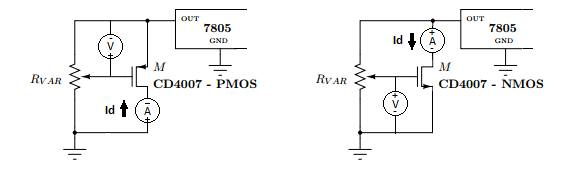
\includegraphics[scale=0.7]{./Imagenes/banco_vg.jpg}
\caption{Circuitos para la medición de la curva de transferencia $i_D$ vs. $V_{GS}$}
 \label{fig:banco_vg}
\end{center}
\end{figure}

Dado que previamente se habían realizado las simulaciones correspondientes a cada circuito se decidió tomar más puntos de medición en los codos de las curvas, es decir donde comienza la saturación del transistor, ya que en esta parte de la curva es donde se produce una mayor variación de $i_D$ con respecto a $v_{GS}$.
Los resultados obtenidos son detallados más adelante donde se realiza una comparación con los valores obtenidos del modelo de \emph{Spice} y un modelo modificado.

\subsubsection{Curva de salida de los transistores: $i_D$ vs. $v_{DS}$ para $v_{GS} = cte$}

En este caso se utilizó el banco de medición detallado en la figura \ref{fig:banco_vd}. Se realizaron mediciones de $i_D$ vs. $v_{DS}$ para las cuales se obtuvieron dos $I_{D_{SAT}}$ distintas, $0,5\unit{mA}$ y $2,5\unit{mA}$  para transistores NMOS,  $-0,5\unit{mA}$ y $-2,5\unit{mA}$ para transistores PMOS.


A partir de los resultados de $V_T$ e $I_{D_{SAT}}$ obtenidos en la medición experimental de la curva $i_D$ vs. $v_{GS}$ se calculó el valor del potenciómetro conectado al \emph{Gate}, con el fin de obtener una tensión del \emph{Gate} para que la corriente de drain en saturación fuera la deseada. 


Una vez fijada la tensión del \emph{Gate} para cada $I_{D_{SAT}}$, se procedió a variar $R_D$, con el fin de alterar la tensión $v_{DS}$  y poder obtener los valores de la curva deseada (manteniendo siempre $v_{GS}$ constante en la obtención de cada curva ).


EL agregado de $R_D$ se debe a que contábamos con una fuente regulada constante de $5\unit{V}$. Por lo tanto al agregar esta resistencia variable, parte de la tensión regulada cae sobre ella y de esta manera se consiguió variar la tensión $v_{DS}$ sobre el transistor. Se calculó el rango en el cual debía variar $R_D$, para que fuera posible relevar tanto la región de codo como la región de saturación de la curva $i_D$ vs. $v_{DS}$.  


Del circuito mostrado en la figura \ref{fig:banco_vd} obtenemos la ecuación \ref{eq:id_vds}. Siendo $V_{DD}= 5\unit{V}$ la salida del regulador de tensión \textbf{LM7805}.

\begin{equation}
i_D =\frac{V_{DD}}{R_D} - \frac{v_{DS}}{R_D}
\label{eq:id_vds}
\end{equation}
 
Se eligió un valor máximo de $R_D$ para el cual se obtuvieron valores de $i_D$ que eran de importancia para el análisis.
Por lo tanto, para $I_{D_{SAT}}=2,5 \unit{mA}$ se eligió $R_{D_{MAX}}$ de $5 \unit{k\Omega}$, ya que corresponde a $i_D = 1 \unit{mA}$ aproximadamente,  de la ecuación \ref{eq:id_vds} se obtiene la aproximación $I_D  \simeq \frac{V_{DD}}{R_D}$.


En el caso de $I_{D_{SAT}}=0,5 \unit{mA}$ se eligió $R_{D_{MAX}} = 15 \unit{k\Omega}$, ya que corresponde a $i_D \simeq 3,5 \unit{mA}$.
Se decidió tomar el valor de $R_{D_{MIN}}=0 \unit{k\Omega}$ que corresponde a $V_{DS}=V_{DD}$ ya que era interesante analizar estos puntos para calcular la pendiente de la recta de $I_D$ en saturación.


\begin{figure}[H] %[h] para here [b] para bottom [t] para top [H]+float para aqui si o si
\begin{center}
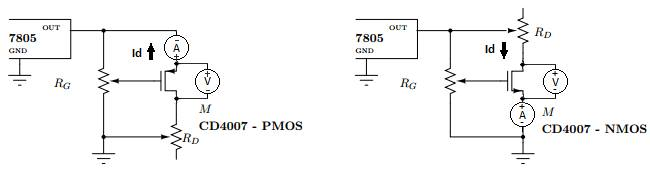
\includegraphics[scale=0.7]{./Imagenes/banco_vd.jpg}
\caption{Circuitos para la medición de la curva de salida  $i_D$ vs $v_{DS}$}
 \label{fig:banco_vd}
\end{center}
\end{figure}

\subsection{Obtención de parámetros}

Una vez obtenidas las curvas experimentales y las curvas simuladas, por métodos numéricos se realizó el ajuste de la recta $y=Ax+B$ a los valores obtenidos de $\sqrt{i_D}$ vs. $v_{GS}$ que cumplen la ecuación \ref{eq:sqrt_id} para los valores $i_D > 0 \unit{mA}$. De esta forma con los parámetros finales de la recta se obtuvieron $k$ y $V_T$.

\begin{equation}
\sqrt{i_D}=\sqrt{k}(v_{GS}-V_T)
\label{eq:sqrt_id}
\end{equation}


Para calcular $\lambda$ y $r_o$ se ajustó la recta con los valores obtenidos de $i_D$ vs. $v_{DS}$ que cumplen la ecuación $i_D=I_{D_{sat}}+\frac{v_{DS}}{r_0}$. Para obtener dichos valores se ajustó la región de las curvas que tenían pendiente constante. De esta forma con los parámetros finales de la recta se obtuvieron $I_{D_{SAT}}$ y $g_o$. Con los que se calculó $r_o = g_o^{-1}$ y $\lambda = \frac{g_o}{I_{D_{SAT}}}$

\subsection{Simulación del modelo modificado}

Se diseño un modelo modificado basado en el modelo de la biblioteca \texttt{CD4007.lib} reemplazando los parámetros $k$, $V_T$ y $\lambda$ obtenido en los ajustes de M1 para NMOS y de M2 para PMOS. Con estos valores se repitieron las simulaciones.

Se debe tener en cuenta que el parámetro $K_P$ de \emph{Spice} no es el mismo $k$ obtenido mediante los ajustes. Puede obtenerse mediante la ecuación \ref{eq:KP} Siendo $\frac{L}{W} = 1$.

\begin{equation}
\displaystyle K_P = k\ 2\ \frac{L}{W}
\label{eq:KP}
\end{equation}

En el caso de las curvas para los PMOS se incluyó la siguiente directiva: 
    
\texttt{.MODEL MiModelo PMOS (LEVEL=1 KP=645.45u VT0=-1.352233 LAMBDA=75.862m)}
    
En el caso de las curvas para los transistores tipo N se incluyó la siguiente directiva:

\texttt{.MODEL MiModelo NMOS (LEVEL=1 KP=755.81u VT0=1.1703 LAMBDA=8.5116m)}


\section{Análisis y comparación de los resultados}

\subsection{Curvas obtenidas}

\subsubsection{PMOS}

\begin{figure}[H] %[h] para here [b] para bottom [t] para top [H]+float para aqui si o si
\begin{center}
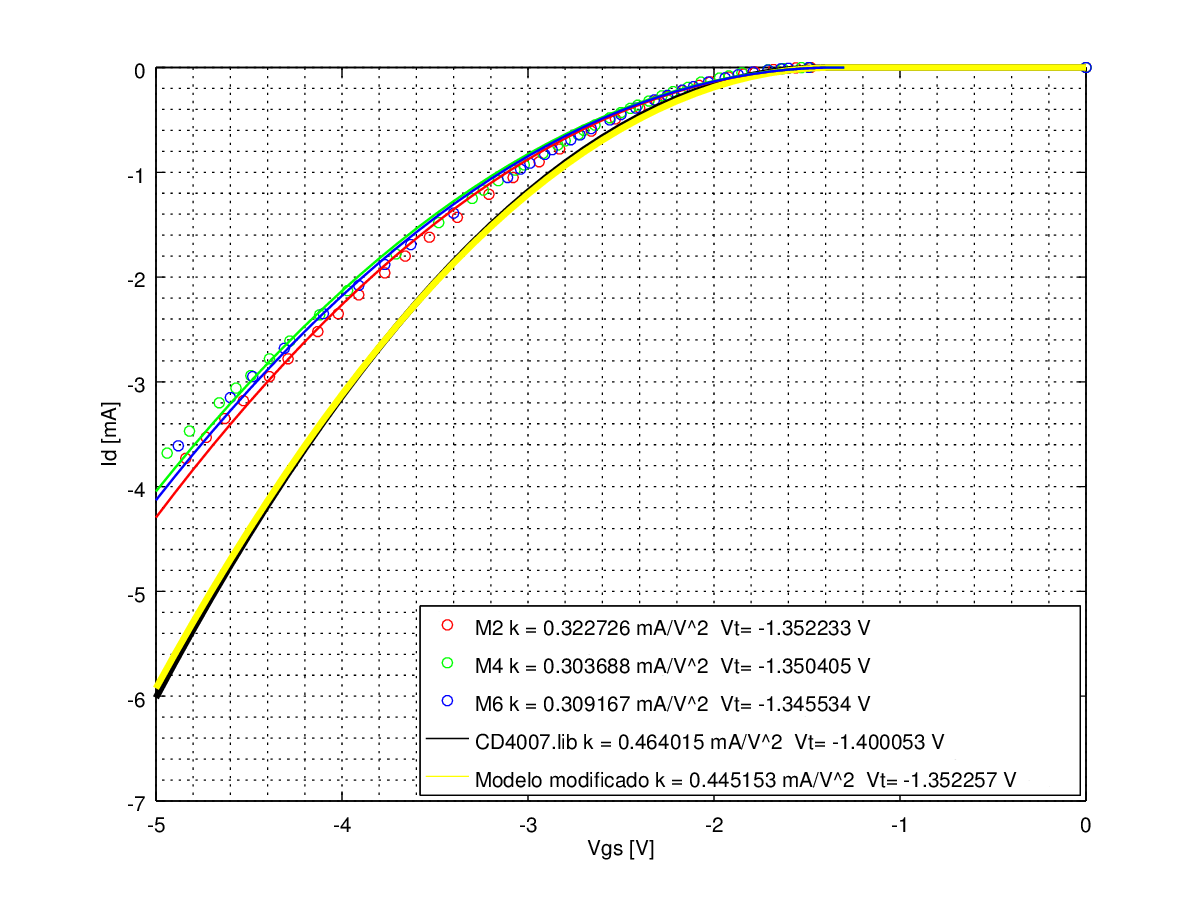
\includegraphics[scale=0.65]{./octave/P_ID_VG.png}
\caption{Curva de transferencia PMOS: $i_D$ vs. $v_{GS}$ para $v_{DS} = -5 \unit{V}$}
 \label{fig:P_ID_VG}
\end{center}
\end{figure}

\begin{figure}[H] %[h] para here [b] para bottom [t] para top [H]+float para aqui si o si
\begin{center}
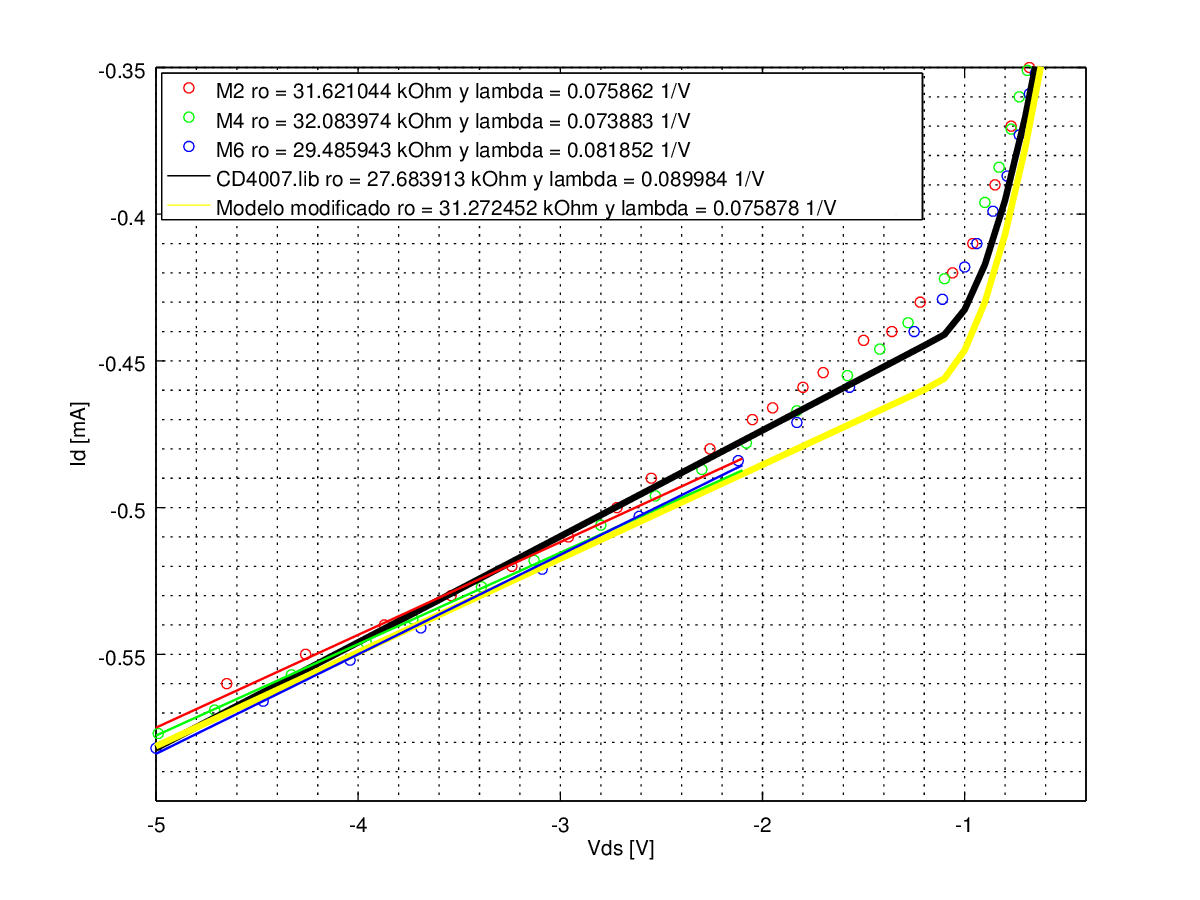
\includegraphics[scale=0.65]{./octave/P_ID_VDS_500.png}
\caption{Curva de salida PMOS: $i_D$ vs. $v_{DS}$ para $I_{D_{SAT}} = -0,5 \unit{mA}$}
 \label{fig:P_ID_VDS_500}
\end{center}
\end{figure}

\begin{figure}[H] %[h] para here [b] para bottom [t] para top [H]+float para aqui si o si
\begin{center}
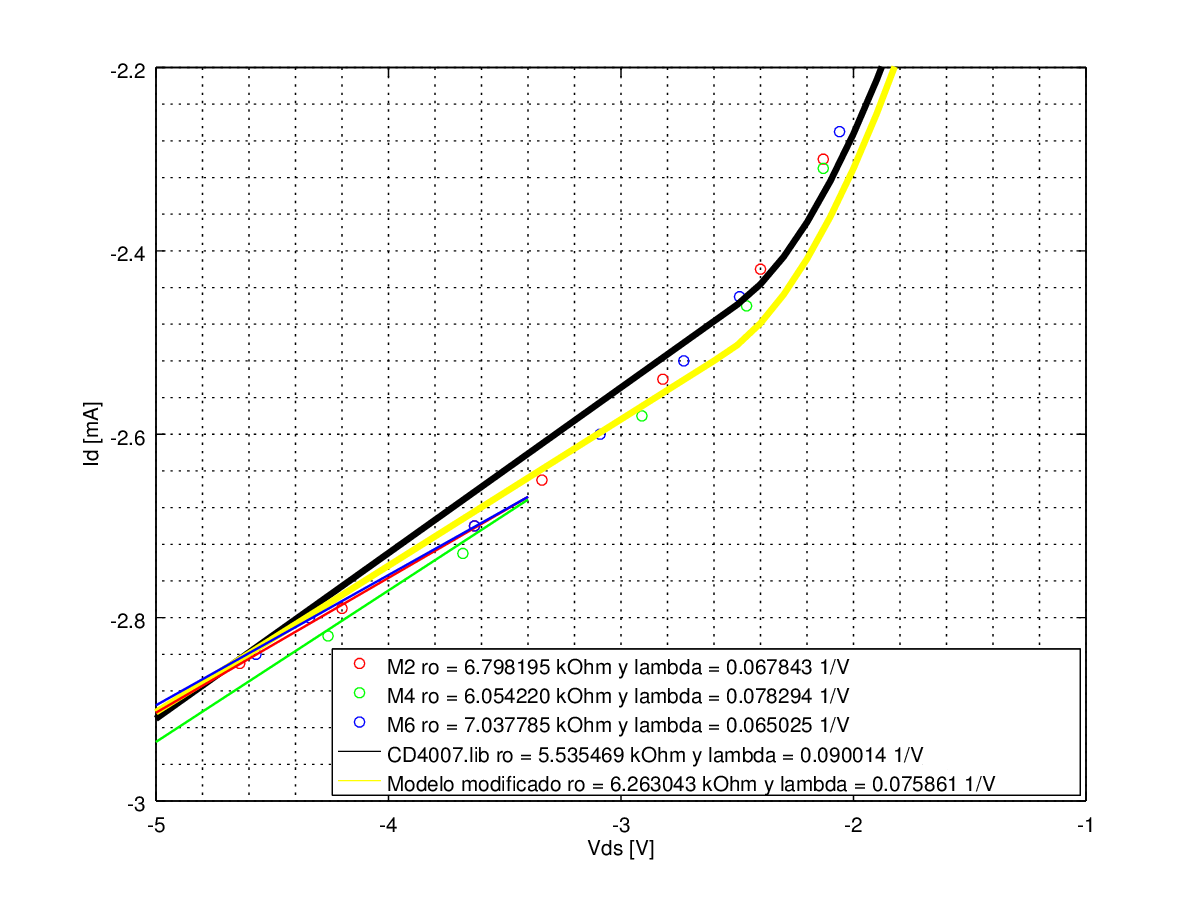
\includegraphics[scale=0.65]{./octave/P_ID_VDS_2500.png}
\caption{Curva de salida PMOS: $i_D$ vs. $v_{DS}$ para $I_{D_{SAT}} = -2,5 \unit{mA}$}
 \label{fig:P_ID_VDS_2500}
\end{center}
\end{figure}

\begin{figure}[H] %[h] para here [b] para bottom [t] para top [H]+float para aqui si o si
\begin{center}
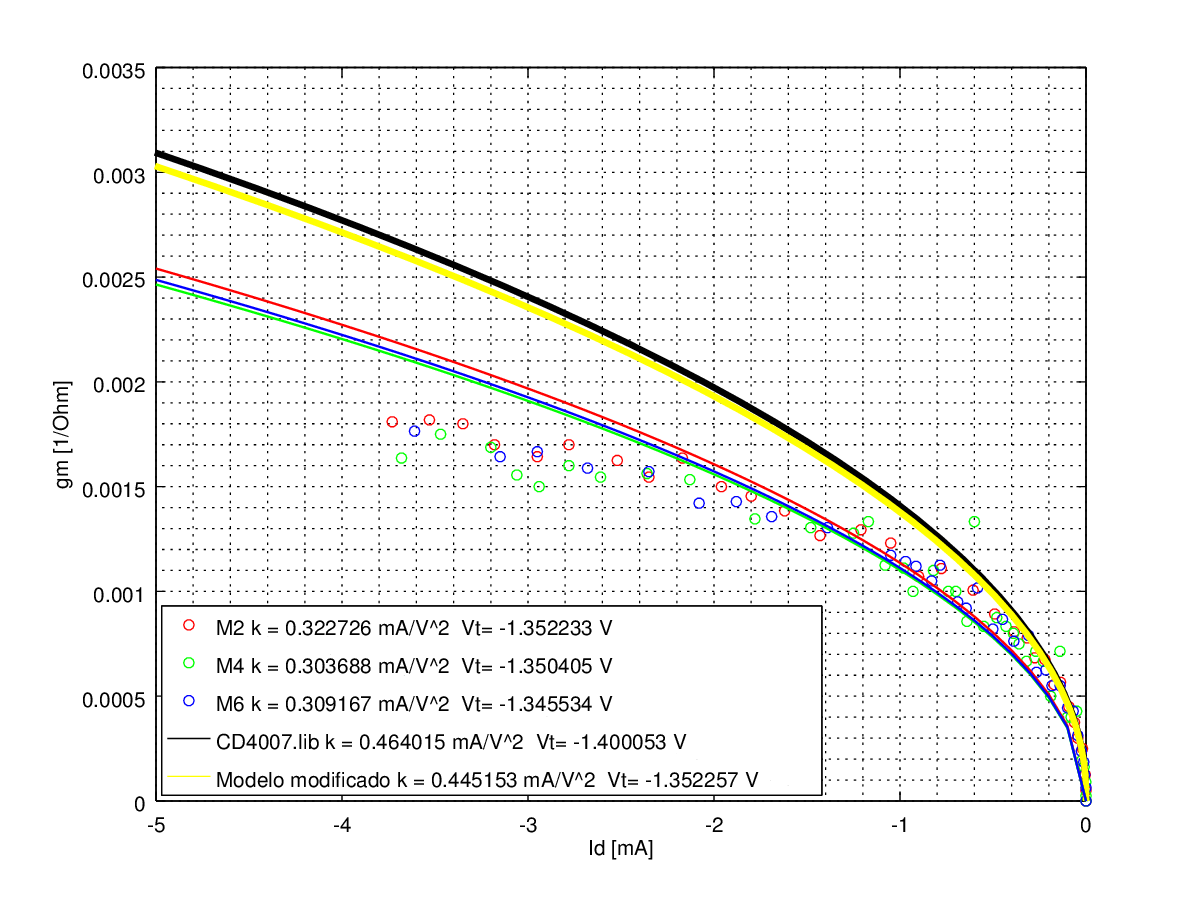
\includegraphics[scale=0.65]{./octave/P_GM_ID.png}
\caption{Curva de transconductancia PMOS: $g_m$ vs. $i_D$}
 \label{fig:P_ID_VDS_500}
\end{center}
\end{figure}

\subsubsection{NMOS}

\begin{figure}[H] %[h] para here [b] para bottom [t] para top [H]+float para aqui si o si
\begin{center}
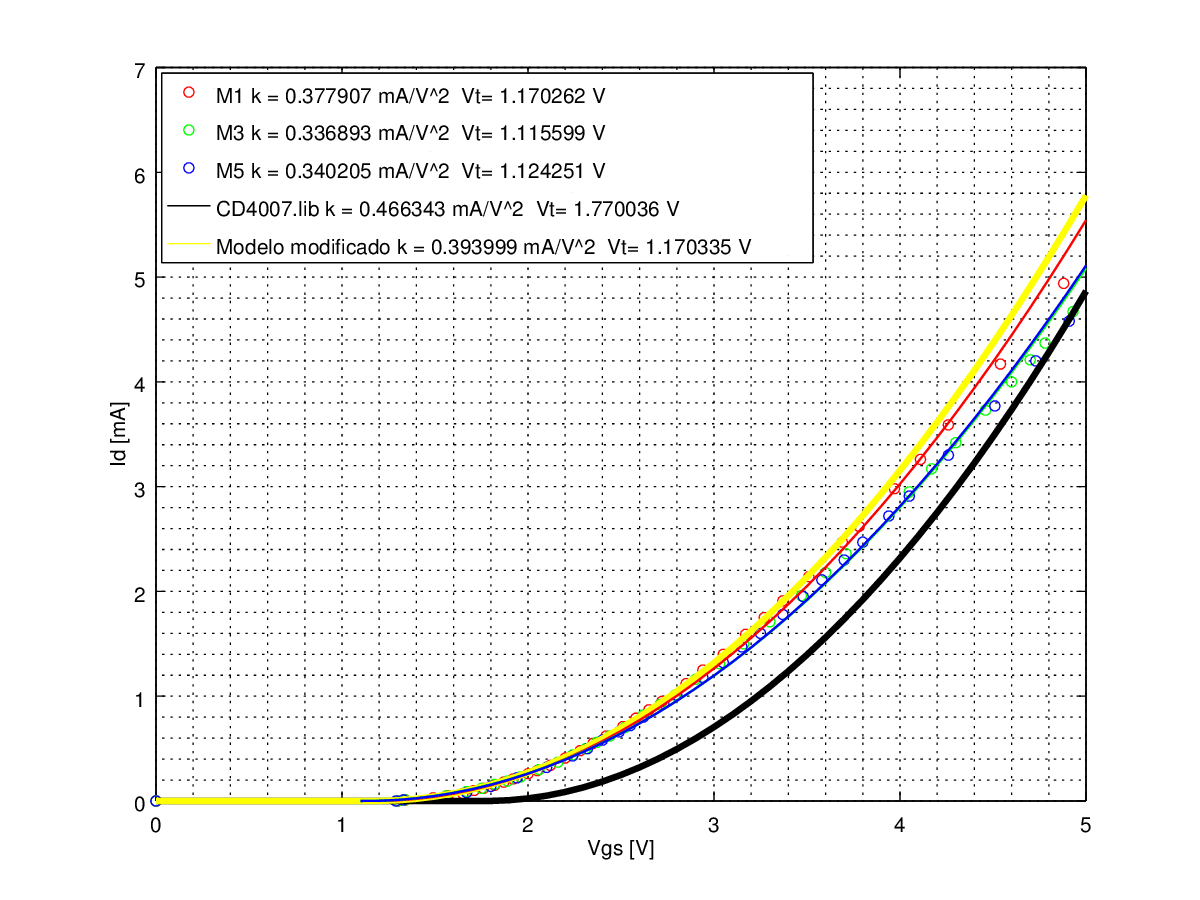
\includegraphics[scale=0.65]{./octave/N_ID_VG.png}
\caption{Curva de transferencia NMOS: $i_D$ vs. $v_{GS}$ para $v_{DS} = 5 \unit{V}$}
 \label{fig:N_ID_VG}
\end{center}
\end{figure}

\begin{figure}[H] %[h] para here [b] para bottom [t] para top [H]+float para aqui si o si
\begin{center}
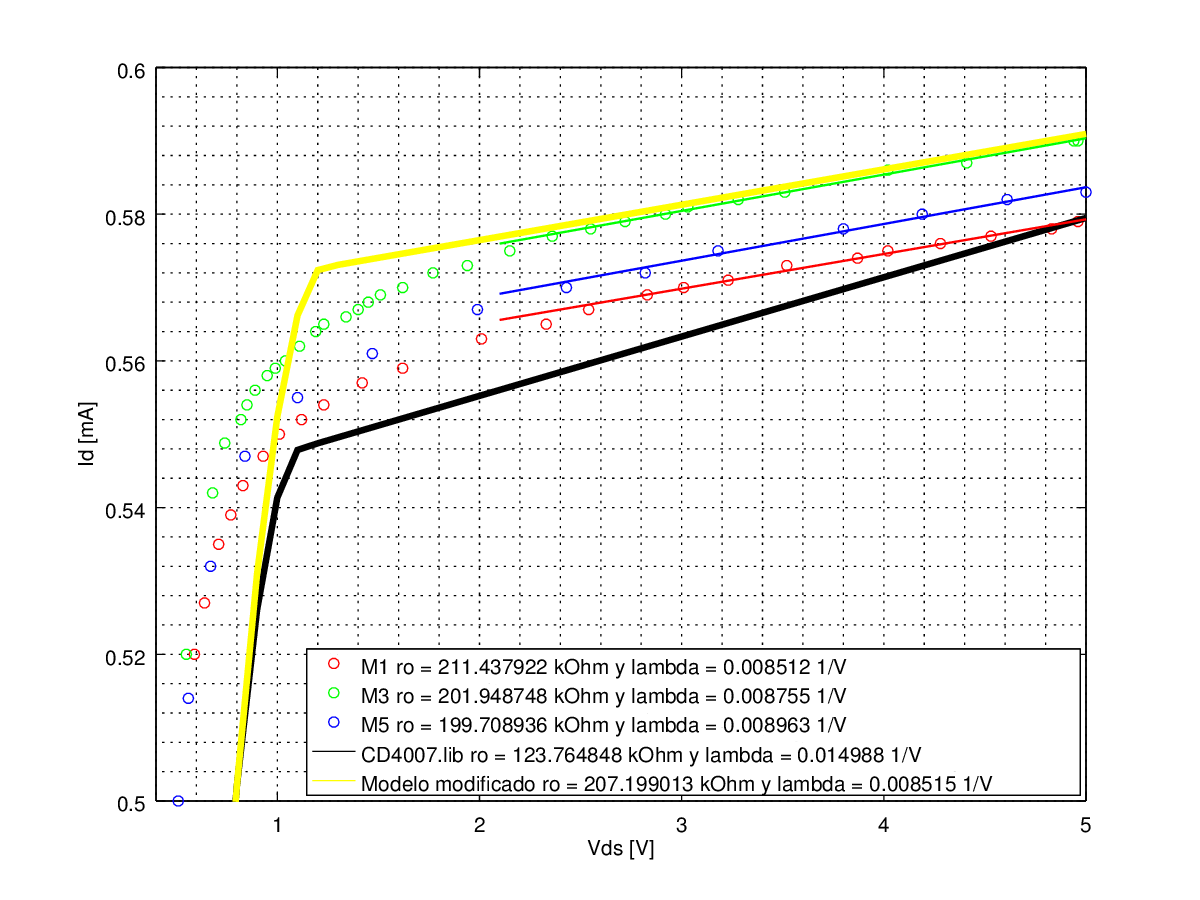
\includegraphics[scale=0.65]{./octave/N_ID_VDS_500.png}
\caption{Curva de salida NMOS: $i_D$ vs. $v_{DS}$ para $I_{D_{SAT}} = 0,5 \unit{mA}$}
 \label{fig:N_ID_VDS_500}
\end{center}
\end{figure}

\begin{figure}[H] %[h] para here [b] para bottom [t] para top [H]+float para aqui si o si
\begin{center}
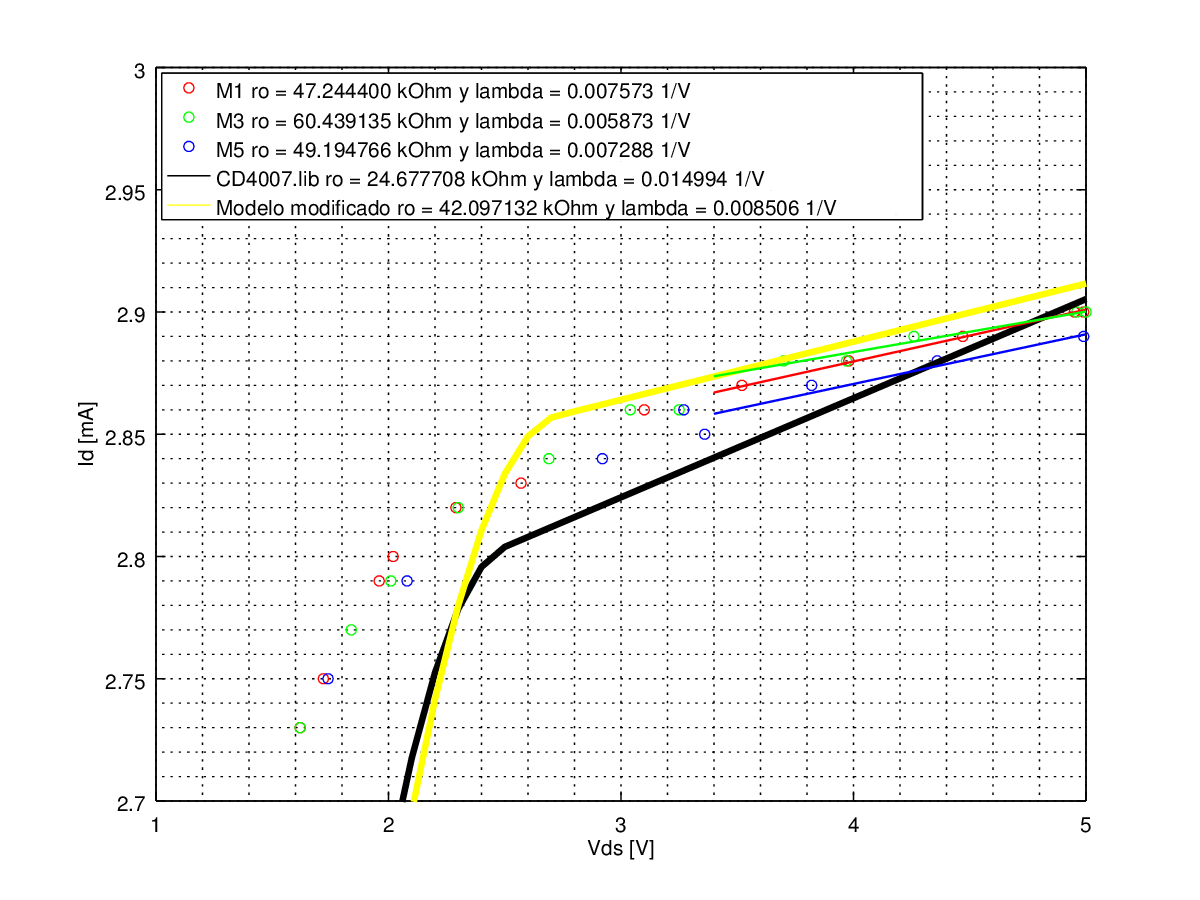
\includegraphics[scale=0.65]{./octave/N_ID_VDS_2500.png}
\caption{Curva de salida NMOS: $i_D$ vs. $v_{DS}$ para $I_{D_{SAT}} = 2,5 \unit{mA}$}
 \label{fig:N_ID_VDS_2500}
\end{center}
\end{figure}

\begin{figure}[H] %[h] para here [b] para bottom [t] para top [H]+float para aqui si o si
\begin{center}
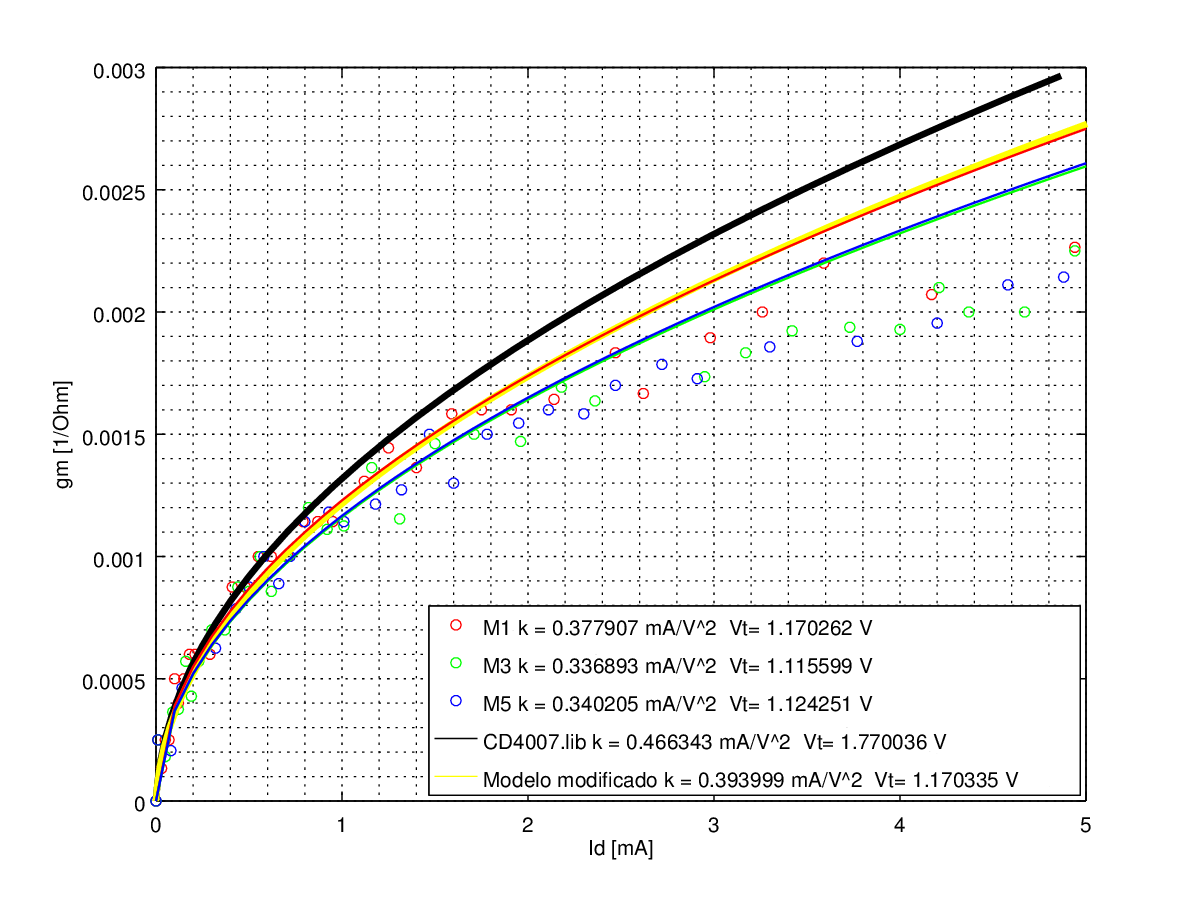
\includegraphics[scale=0.65]{./octave/N_GM_ID.png}
\caption{Curva de transconductancia NMOS: $g_m$ vs. $i_D$}
 \label{fig:N_GM_ID}
\end{center}
\end{figure}

\subsection{Comparación de los resultados}

En la tabla \ref{table:comparacion} se muestran las diferencias relativas de los transistores M1, M2 y los transistores de la biblioteca \texttt{CD4007.lib} respecto al modelo modificado NMOS y PMOS respectivamente.

Se comparan los parámetros de los transistores M1 y el modelo modificado  NMOS y el transistor M2 con el modelo modificado PMOS, ya que los modelos modificados fueron diseñados con los parámetros de M1 y M2 para los NMOS y PMOS respectivamente.\\
También son comparados los parámetros de los transistores de la biblioteca \texttt{CD4007.lib} con el modelo modificado tanto para transistores NMOS como PMOS, ya que el modelo modificado fue diseñado en base al modelo de la biblioteca \texttt{CD4007.lib} solo modificando los parámetros $k$, $V_T$ y $\lambda$ así podremos estudiar la influencia de dichos parámetros en las simulaciones.


\begin{table}[H]
\centering
\begin{tabular}{c|c|c|c|c|c|l}
\cline{2-6}
& Transistor & \multicolumn{2}{ c| }{PMOS} & \multicolumn{2}{ c| }{NMOS} \\ \cline{2-6}

& $X$ & M2 & \texttt{CD4007.lib} & M1 & \texttt{CD4007.lib} \\ \cline{2-6}

& $\displaystyle \abs{\frac{k_{X} - k_{modelo\ modificado}}{k_{modelo\ modificado}}} \ 100 \%$  & 
$27,5 \%$ & $ 4,2\%$ & $ 4,1\%$ & $ 18,4\%$ & \\ \cline{2-6}

& $\displaystyle \abs{\frac{V_{T_{X}} - V_{T_{modelo\ modificado}}}{V_{T_{modelo\ modificado}}}} \ 100 \%$ & $ 0,001\%$ & $ 3,5\%$ & $  0,006\%$ & $ 51,2\%$ & \\ \cline{1-6}

\multicolumn{1}{ |c  }{\multirow{2}{*}{$I_{D_{SAT}} \simeq 0,5 \unit{mA}$} } & \multicolumn{1}{ |c| }{ $\displaystyle \abs{\frac{r_{o_{X}} - r_{o_{modelo\ modificado}}}{r_{o_{modelo\ modificado}}}} \ 100 \%$} & $1,1 \%$ & $ 11,5\%$ & $ 2,0 \%$ & $ 40,3\%$ &     \\ \cline{2-6}

\multicolumn{1}{ |c  }{}                        & \multicolumn{1}{ |c| }{$ \displaystyle \abs{\frac{\lambda_{X} - \lambda_{modelo\ modificado}}{\lambda_{modelo\ modificado}}} \ 100 \%$} & $ 0,02\%$ & $ 18,6\%$ & $ 0,04\%$ & $ 76,0\%$ &     \\ \cline{1-6}

\multicolumn{1}{ |c  }{\multirow{2}{*}{$I_{D_{SAT}} \simeq 2,5 \unit{mA}$} } & \multicolumn{1}{ |c| }{ $\displaystyle \abs{\frac{r_{o_{X}} - r_{o_{modelo\ modificado}}}{r_{o_{modelo\ modificado}}}} \ 100 \%$} & $8,5 \%$ & $ 11,6\%$ & $ 12,2\%$ & $ 41,4\%$ &  \\ \cline{2-6}

\multicolumn{1}{ |c  }{}                        & \multicolumn{1}{ |c| }{$ \displaystyle \abs{\frac{\lambda_{X} - \lambda_{modelo\ modificado}}{\lambda_{modelo\ modificado}}} \ 100 \%$} & $ 10,6\%$ & $ 18,7\%$ & $ 11,0 \%$ & $ 76,2 \%$ &  \\ \cline{1-6}

\end{tabular}
\caption{Comparación de los parámetros principales respecto al modelo modificado}
\label{table:comparacion}
\end{table}

A continuación se listan las principales relaciones encontradas entre las curvas y sus parámetros:

\begin{itemize}

\item En la mayoría de las comparaciones de los parámetros se obtiene menor diferencia entre M1 con su modelo modificado y M2 con  su modelo modificado a comparación de las diferencias entre los modelos modificados y los transistores de la biblioteca \texttt{CD4007.lib}. Esto demuestra que tienen mas influencia en el comportamiento del transistor los parámetros modificados de la biblioteca \texttt{CD4007.lib} que el resto de los parámetros que la componen.

\item Como se puede apreciar en las curvas de salida para los transistores NMOS, los resultados en el régimen de \emph{saturación} son compatibles.
Y en régimen \emph{triodo}  presenta un comportamiento distinto  a pesar de tener una diferencia del $4,1\%$ para el valor de $k$ y una diferencia del $0,006\%$ para el valor de $V_T$  en los parámetros de M1 respecto al modelo modificado. Esto se puede deber a que la ecuación de la corriente en \emph{triodo}(ecuación \ref{eq:I_D_triodo}) sea distinta a las curvas de salida de los transistores medidos o bien \emph{Spice} no utiliza dicha ecuación en el régimen \emph{triodo}.

\begin{equation}
I_D = 2 k \Big(V_{GS} - V_T - \frac{V_{DS}}{2}\Big) V_{DS}
\label{eq:I_D_triodo}
\end{equation}

\item Las curvas de $g_m$ vs. $i_D$ encontramos que a medida que $i_D$ crece los valores de $g_m$ obtenidos con las mediciones realizadas  son aproximadamente un $22,2\%$ mas pequeño que los valores obtenidos mediante cálculos teóricos.

\item El transistor M2 encontramos una diferencia mayor entre su parámetro $k$ y el del modelo modificado. Esto puede deberse a que en la biblioteca \texttt{CD4007.lib} $\frac{L}{W}$ sea distinto de 1 y así el $k$ obtenido mediante el ajuste será distinto.

\item Tanto para las simulaciones en \emph{Spice} como para las curvas medidas los $\lambda$ de los transistores NMOS son de un orden de magnitud comparado con los $\lambda$ de los transistores PMOS. Comparando el transistor M1 y M2 se llega a que $\lambda_{M2}$ es un $88,5\%$ mas grande que $\lambda_{M1}$. 

\end{itemize}

\subsection{Problemas a resolver}

Una vez obtenidos los parámetros característicos, elegimos las curvas del transistor M1 y M2 para resolver los siguientes problemas:

\begin{enumerate}
\item   A partir de la curva de transferencia de uno de los transistores PMOS, encuentre el valor de
$V_{GS}$ y el valor de las resistencias del divisor resistivo en el \emph{Gate} para obtener una corriente $I_D=-1,5 \unit{V}$.

De la Figura \ref{fig:P_ID_VG} para $I_D=-1,5 \unit{V}$ se obtiene $V_{GS} = -3,6 \unit{V}$.

Finalmente del divisor resistivo formado por las tensiones $V_{GS} = -3,6 \unit{V}$ y $V_{DD} = -5 \unit{V}$ (Figura \ref{circuito:divisor_tension_gate}) y teniendo en cuenta que $R_{G_1}$ y $R_{G_2}$ forman el potenciómetro $R_G = 20k\Omega$ se obtienen las siguientes ecuaciones:

\[ \displaystyle -3,6 \unit{V} = \frac{R_{G_2}}{R_{G_1} + R_{G_2}} \ (-5 \unit{V}) \ \ \ \ \ \ \ \ \ \ \ \ \ \  R_{G_1} + R_{G_2} = 20 \unit{k\Omega}\]

Despejando $ R_{G_1}$ y $R_{G_2}$ se llega a los siguientes resultados:

\[ \displaystyle R_{G_1} = 5,6 \unit{k\Omega} \ \ \ \ \ \ \ \ \ \ R_{G_2} = 14,4 \unit{k\Omega} \]


\begin{figure}[H]
\centering
\begin{circuitikz}[american]\shorthandoff{>}
\draw 
(0,0.5) node[ground]{} 
to [R, l = $R_{G_2}$] (0,2)
to [R, l = $R_{G_1}$] (0,4)
(0,2) to [short, -o] (1,2) node[anchor=south]{$V_{GS}$} 
(0,4) to [short, -o] (-1,4) node[anchor=south]{$V_{DD}$} 
;\end{circuitikz}
\caption{divisor de tensión}
\label{circuito:divisor_tension_gate}
\end{figure}


\item  Para la curva de salida de los transistores NMOS, teniendo en cuenta que $R_D$ es un potenciómetro de $20 \unit{k\Omega}$, ¿cuál sería la mínima corriente que puede medir?

La menor corriente se obtiene en el régimen \emph{triodo} por lo tanto:

\[ \displaystyle I_D = 2 k \Big(V_{GS} - V_T - \frac{V_{DS}}{2}\Big) V_{DS} \]


Del circuito para NMOS mostrado en la Figura \ref{fig:banco_vd} obtenemos la siguiente ecuación:
 
 \begin{equation}
I_D = \frac{V_{DD} - V_{DS}}{R_D} 
\label{eq:I_D_circuito}
\end{equation}

Siendo $V_{DD} = 5\unit{V}$ la salida del regulador de tensión \textbf{LM7805}.

Encontramos una relación inversa entre $I_D$ y $R_D$ de la ecuación \ref{eq:I_D_circuito}. Por lo tanto $I_D$ alcanzará si valor mínimo a mayor valor de $R_D = 20 \unit{k\Omega}$. 

Reemplazando la ecuación \ref{eq:I_D_triodo} en \ref{eq:I_D_circuito} se obtiene la siguiente ecuación cuadrática de $V_{DS}$:

\begin{equation}
0 = V_{DS}^2 - V_{DS} \left( 2 (V_{GS} - V_T) + \frac{1}{k\ R_D} \right) + \frac{V_{DD}}{k\ R_D}
\end{equation}

Una vez calculado $V_{DS}$  despejamos $I_D$ de la ecuación \ref{eq:I_D_circuito}.

A continuación se calcula $I_{DS}$ y $V_{DS}$ con los parámetros del transistor \textbf{M1} para las dos tensiones de $V_{GS}$ utilizadas en el trabajo: 

\begin{itemize}
\item $V_{GS} = 2,36\unit{V}\ (I_{D_{SAT}} \simeq 0,5 \unit{mA})$: $V_{DS} = 0,3 \unit{V}$ \ \ \ $I_{D_{min}} = 0,235 \unit{mA}$
\item $V_{GS} = 3,91\unit{V}\ (I_{D_{SAT}} \simeq 2,5 \unit{mA})$: $V_{DS} = 0,12 \unit{V}$ \ \ $I_{D_{min}} = 0,244 \unit{mA}$
\end{itemize}



\item  Para el caso anterior, suponiendo al transistor polarizado de forma tal que $I_{D_{SAT}} = 2,5 \unit{mA}$, ¿cuál es el valor de la resistencia $R_D$ cuando $V_{DS} = 2,5 \unit{V}$?

De la ecuación \ref{eq:I_D_circuito} se despeja $R_D$ y se obtiene:

\[ \displaystyle R_D = \frac{V_{DD} - V_{DS}}{I_D} = \frac{5 \unit{V} - 2,5\unit{V} }{2,5 \unit{mA}} = 1\unit{k\Omega} \]

\item  Si mantengo ese valor de resistencia de \emph{Drain}, pero ahora se cambia $V_{GS}$ de forma tal que
$I_{D_{SAT}} = 0,5 \unit{mA}$, ¿cómo será el nuevo valor de $V_{DS}$ , igual, mayor o menor? Justificar a partir de la recta de carga.

De la ecuación \ref{eq:I_D_circuito} se despeja $V_{DS}$ y se obtiene:

\[ \displaystyle V_{DS} = V_{DD} - I_D\ R_D = 5 \unit{V} - 0,5 \unit{mA} \ 1 \unit{k\Omega} = 4,5 \unit{V} \]

Siendo el $V_{DS}$ calculado mayor al del ejercicio 3.

\item  Para el caso 3, ¿cuál es el máximo valor de $R_D$ de forma tal que el transistor se encuentre en
saturación? ¿Cuál es la tensión $V_{DS}$ en ese caso?

De la ecuación de la corriente de saturación $I_D = k\ (V_{GS} - V_T)^2$ se  calcula $V_{GS}$:

\[ \displaystyle V_{GS} = \sqrt{\frac{I_D}{k}} + V_T = 3,7 \unit{V}\]

Planteando las condiciones de \emph{saturación}: $V_{GS} > V_T$\ \ \ $V_{GD} > V_T$ \ \ \  $V_{DS} > 0 \unit{V}$

Se obtienen los valores de $V_{DS}$ para los cuales se cumplen las condiciones de \emph{saturación}:

\[ \displaystyle  V_{GD} = V_{GS} - V_{DS} < V_T   \Longrightarrow V_{DS} > V_{GS} - V_{T} = 2,5 \unit{V} \]
 
De la ecuación \ref{eq:I_D_circuito} se encuentra que $R_D$ alcanza su máximo valor a menor $V_{DS}$. Siendo $V_{DS} = 2,5\unit{V}$ el mínimo valor para seguir en \emph{saturación}.
Despejando $R_D$ obtenemos:

\[ \displaystyle R_D = \frac{V_{DD} - V_{DS}}{I_D} = \frac{5 \unit{V} - 2,5\unit{V} }{2,5 \unit{mA}} = 1\unit{k\Omega} \]

\end{enumerate}

\section{Conclusiones}

Con la realización de este trabajo práctico se pudo apreciar lo bien
que se aproxima el modelo matemático de los transistores MOSFET. Se
pudo cuantificar las diferencias entre transistores del mismo modelo,
y a su vez comparar estos valores con los provenientes de la
simulación con \emph{Spice}.

En base al trabajo realizado se concluye que el parámetro $\lambda$ es menor para los transistores NMOS que los PMOS.

Las ecuaciones comúnmente utilizadas para el régimen de \emph{saturación} tiene un comportamiento compatible con las curvas obtenidas experimentalmente y simuladas. Pero en el régimen de \emph{saturación} su comportamiento difiere.

Los valores de $g_m$ obtenidos mediante las curvas medidas difieren de los obtenidos mediante cálculos teóricos a medida que $i_D$ aumenta.

Una observación importante es que la resistencia de salida disminuye
al aumentar la corriente de saturación. De aquí se concluye que esta es una propiedad
importante del transistor ya que permite controlar la resistencia que
percibe algún circuito externo conectado al transistor. También se
puede concluir que en régimen de saturación, el MOSFET puede actuar
como un elemento que otorga una corriente aproximadamente constante al \emph{Drain}, siempre y cuando la tensión de Drain no caiga por debajo del punto de saturación.

\end{document}

\grid
